The interplanetary transfer time has a big impact on the design. The interplanetary transfer time determines for instance the mass of food for the astronauts, the amount of radiation to endure, how much they need to exercise and more. Keeping the transfer time short will minimise these problems. However it will also increase the $\Delta\gls{sym:V}$-budget needed for the launcher. 

\begin{figure}[h]
	\centering
	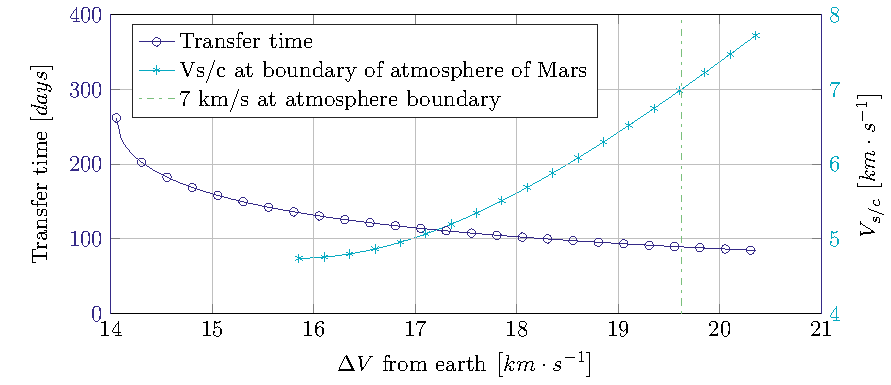
\includegraphics[width=0.95\textwidth]{Figure/Inter_transfer/transfer_time.pdf}
	\caption[Interplanetary transfer time and entry velocity versus $\Delta\gls{sym:V}$]{Interplanetary transfer time (left) and entry velocity (right) versus $\Delta\gls{sym:V}$}
	\label{fig:inter_time}
\end{figure}

The most efficient transfer with respect to the $\Delta\gls{sym:V}$-budget consists of a Hohmann transfer orbit. This would take approximately 262 days. This time is the longest of all orbits to Mars with a direct transfer. One of the mission requirements is the entry velocity of 7 $\left[km \cdot s^{-1}\right]$. This velocity is fully determined by the $\Delta \gls{sym:V}$ budget and thereby corresponds to the transfer time. In Figure \ref{fig:inter_time} this relation is visualised. As can be seen to arrive with the required velocity a $\Delta \gls{sym:V}$ of $19.62$ $\left[km \cdot s^{-1}\right]$ is required, which corresponds to a transfer time of $89.3$ $\left[days\right]$. The corresponding orbit is shown in Figure \ref{fig:inter_orbit}.

\begin{figure}[h]
	\centering
	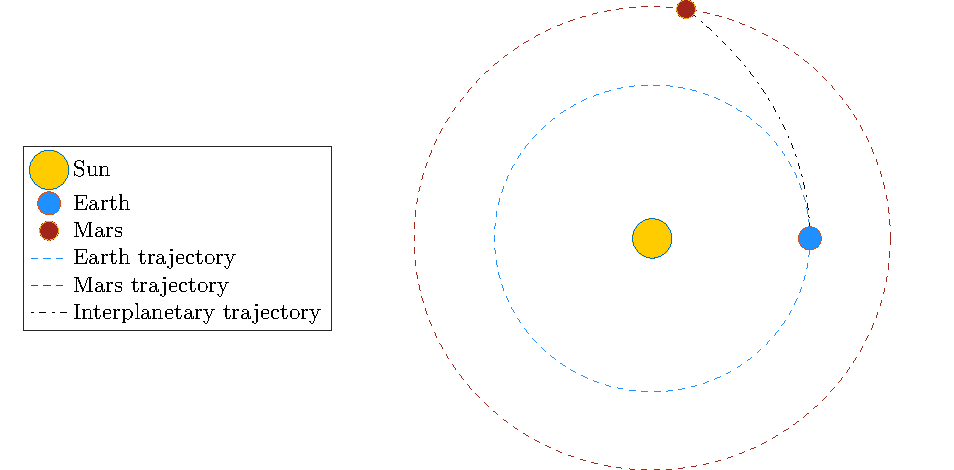
\includegraphics[width=0.95\textwidth]{Figure/Inter_transfer/orbits.pdf}
	\caption[Visualisation of the interplanetary transfer orbit]{Visualisation of the interplanetary transfer orbit. Planets not to scale}
	\label{fig:inter_orbit}
\end{figure}
